% SNT - 2019
% (C) Stéphane Colomban (CC : sd-by-sa)




\documentclass[a4paper,10pt]{article}
\usepackage[rgb]{xcolor}
\usepackage[utf8]{inputenc}
\usepackage[T1]{fontenc}
\usepackage[frenchb]{babel}
\usepackage{mathrsfs, amsmath, amssymb}
\usepackage{times,mathptmx}
\DeclareSymbolFont{lmodern}{U}{euex}{m}{n}
\DeclareMathSymbol\infty \mathord{lmodern}{"31}
\usepackage[scaled=0.875]{helvet} % ss
\usepackage{textcomp}
\usepackage{dsfont} % pour les symboles des ensembles
\usepackage[left=2cm,right=2cm,top=0.5cm,bottom=2cm]{geometry}
\usepackage{fancyhdr} 
\fancyhf{}
\setlength{\headheight}{26pt}
\setlength{\footskip}{18pt}
\renewcommand {\headrulewidth}{0pt}
\renewcommand {\footrulewidth}{1pt}

\usepackage{hyperxmp}
\usepackage{listings}
%\usepackage[colorlinks=true,pdfstartview=FitV,linkcolor=blue,citecolor=blue,urlcolor=blue]{hyperref}
\pagestyle{fancy}
\usepackage {array}
\usepackage{tabularx}
\usepackage{multirow}
\usepackage{fltpoint}
\usepackage{pstricks,pst-all,pstricks-add,pst-tree,pst-3dplot,pst-func}
\usepackage{ifthen}
\usepackage{calc}
\usepackage{esvect}
\usepackage[np]{numprint}
\usepackage{pgf}
\usepackage{mathrsfs}
\usepackage{tikz}
\usetikzlibrary{arrows}
\usetikzlibrary[patterns]
\usetikzlibrary{shapes.misc}
\usetikzlibrary{decorations.pathmorphing,calc,shapes,shapes.geometric,patterns}
\setlength{\parindent}{0mm}
\usepackage [alwaysadjust]{paralist}
\usepackage{times,tcolorbox}
\usepackage{luatex85}
\usepackage{listings}
\usepackage{hyperref}

\usepackage{wrapfig}

\hypersetup{
    colorlinks=true,
    linkcolor=blue,
    filecolor=magenta,      
    urlcolor=blue
}
    
    
\setdefaultenum {1.}{a)}{}{}
\hyphenpenalty 10000 
\renewcommand*{\tabularxcolumn}[1]{m{#1}} 
\newcommand{\Oij}{$\left( {{\mathrm{O}};\vec i,\vec j} \right)$}
\newcommand{\Oijk}{$\left( {{\mathrm{O}};\vec i,\vec j ,\vec k} \right)$}
\newcommand{\euro}{\texteuro{}}
\newcommand{\R}{\mathds {R}}
\newcommand{\N}{\mathds {N}}
\newcommand{\Z}{\mathds {Z}}
\newcommand{\Q}{\mathds {Q}}
\newcommand{\e}{\mathrm {e}}
\newcommand{\dd}{\,\mathrm{d}}

\newcommand\pts[1][]{ \textcolor{red} { \hfill #1 pts}} 
\newcommand\pt[1][]{ \textcolor{red} { \hfill #1 pt}} 

\DecimalMathComma
\definecolor{jaune}{rgb} {0.9529,0.9215,0.04705}
\definecolor{bleu}{rgb} {0,0.3725,0.698}
\definecolor{rouge}{rgb} {0.9294,0.1529,0.1411} 
\definecolor{bleuvif}{rgb} {0.01569,0.12941,0.25098}
\definecolor{orange}{rgb} {.9,0.4216,0.06} 
\definecolor{bleuclair}{rgb} {0.2,0.9,1}
\definecolor{vertclair}{rgb} {0.9,1,.8}
\definecolor{vert}{rgb} {0.1,0.6,0.1}
%%%%%%%%%%%%%%%%%%%%%%%%%%%%%%%%%%%%%%%%%%%%%%%%%%%%%%%%%%%%%%%%%%%%%%%%%%%%%%
\newcommand \SNT[3]{

\begin{minipage}{3cm}
\begin{flushleft}
\begin{tikzpicture}[line cap=round,line join=round,>=triangle 45,x=.5cm,y=.5cm]

\draw [color=black, fill=bleuvif]  (0.,0.) rectangle (7,5) ;
\draw [color=black, fill=bleuclair]  (0.05,3.5) rectangle (6.95,4.95) ;

\draw [color=black] (3.5,3.5) node[above] {\textbf{{\Large SNT -- ELLA }}};
\draw [color=white] (3.5,2) node[above] { \textbf{\textsc{#1}}};
\draw [color=white] (3.5,1) node[above] { \textbf{\textsc{#2}}};
\end{tikzpicture}
\end{flushleft}
\end{minipage}
\begin{minipage}{15cm}

  \begin{center} 
   
  \textbf{\textcolor{black}{{\textsc{\Large #3 }}}}\\ 

  \end{center}
\end{minipage}

  
  }


%%%%%%%%%%%%%%%%%%%%%%%%%%%%%%%%%%%%%%%%%%%%%%%%%%%%%%%%%%%%%%%%%%%%%%%%%%%%%%  
\newtcbox{\boitearrondie}{colframe=black, colback=jaune, boxrule=1pt, arc=4pt,
  boxsep=2pt,left=10pt,right=10pt,top=10pt,bottom=10pt}

\newtcbox{\boitecarree}{colframe=red!50, colback=red!10, boxrule=1pt, arc=0pt,
boxsep=2pt,left=10pt,right=10pt,top=10pt,bottom=10pt}

%%%%%%%%%%%%%%%%%%%%%%%%%%%%%%%%%%%%%%%%%%%%%%%%%%%%%%%%%%%%%%%%%%%%%%%%%%%%%%
\newcommand \remarque[3]{
     \begin{tikzpicture}[line cap=round,line join=round,>=triangle 45,x=.07cm,y=.07cm]
       
       \draw[color=red,ultra thick, fill=black] (11,0) node[anchor=west, scale=.8, right] {\Large \color{ #1!} \textsc{\textbf{#3}}};
     \draw[color=#1!110,ultra thick, fill=#1!75](0,0) circle (6);
        {\clip (0,0) circle (12);
       
		   
        \draw[color=white,ultra thick, fill=white] (0,0) node[scale=1] {\huge  \textbf{#2}};
        }
        
  \end{tikzpicture}
}


%%%%%%%%%%%%%%%%%%%%%%%%%%%%%%%%%%%%%%%%%%%%%%%%%%%%%%%%%%%%%%%%%%%%%%%%%%%%%%


%%%%%%%%%%%%%%%%%%%%%%%%%%%%%%%%%%%%%%%%%%%%%%%%%%%%%%%%%%%%%%%%%%%%%%%%%%%%%%
\newcommand\cadre[1]{
\boitearrondie{
\begin{minipage}{\textwidth-30pt}
#1
\end{minipage}
}
}

%%%%%%%%%%%%%%%%%%%%%%%%%%%%%%%%%%%%%%
\newcommand\cadrecarre[1]{
\boitecarree{
\begin{minipage}{\textwidth-30pt}
#1
\end{minipage}
}
}

%%%%%%%%%%%%%%%%%%%%%%%%%%%%%%%%%%%%%%
%%%%%%%%%%%%%%%%%%%%%%%%%%%%%%%%%%%%%%%% 
% Programme en Python
 
\lstset{
backgroundcolor=\color{vertclair!60},
frame=single,
rulecolor=\color{vertclair},
framexleftmargin=2em,
framexbottommargin=1pt,
framextopmargin=1pt,
frame=tb,
%keepspaces=t
language=Python,
numbersep=1em,
showspaces=false,
showtabs=false,
showstringspaces=false,
tabsize=4,
% Basic
basicstyle=\ttfamily\footnotesize\bfseries,
% Strings
stringstyle=\color{red}\bfseries,
morecomment=[s][\color{red}]{"""}{"""},
morecomment=[s][\color{red}]{'''}{'''},
%% keywords
keywordstyle={\textbf{\color{black}\bfseries}},
% additional keywords
keywordstyle={[2]\color{blue}},
commentstyle=\color{darkgray}\ttfamily,  extendedchars=true,
    literate=
    {á}{{\'a}}1 {é}{{\'e}}1 {í}{{\'i}}1 {ó}{{\'o}}1 {ú}{{\'u}}1
    {Á}{{\'A}}1 {É}{{\'E}}1 {Í}{{\'I}}1 {Ó}{{\'O}}1 {Ú}{{\'U}}1
    {à}{{\`a}}1 {è}{{\`e}}1 {ì}{{\`i}}1 {ò}{{\`o}}1 {ù}{{\`u}}1
    {À}{{\`A}}1 {È}{{\'E}}1 {Ì}{{\`I}}1 {Ò}{{\`O}}1 {Ù}{{\`U}}1
    {ä}{{\"a}}1 {ë}{{\"e}}1 {ï}{{\"i}}1 {ö}{{\"o}}1 {ü}{{\"u}}1
    {Ä}{{\"A}}1 {Ë}{{\"E}}1 {Ï}{{\"I}}1 {Ö}{{\"O}}1 {Ü}{{\"U}}1
    {â}{{\^a}}1 {ê}{{\^e}}1 {î}{{\^i}}1 {ô}{{\^o}}1 {û}{{\^u}}1
    {Â}{{\^A}}1 {Ê}{{\^E}}1 {Î}{{\^I}}1 {Ô}{{\^O}}1 {Û}{{\^U}}1
    {œ}{{\oe}}1 {Œ}{{\OE}}1 {æ}{{\ae}}1 {Æ}{{\AE}}1 {ß}{{\ss}}1
    {ç}{{\c c}}1 {Ç}{{\c C}}1 {ø}{{\o}}1 {å}{{\r a}}1 {Å}{{\r A}}1
    {€}{{\EUR}}1 {£}{{\pounds}}1
}



\lfoot{ \vspace{-0.5cm }\copyright \quad  S. COLOMBAN - 2019}
\rfoot{ 
\includegraphics[width=1.8cm]{by-nc-sa.eu.eps} }
\begin{document}

\SNT{Cartographie}{Géolocalisation}{Séance 2 - Analyse des données GPS}

\bigskip
{\large \textbf{Partie 1 : Interprétation de la trame d'un GPS }}
\hrulefill

 

\remarque{orange}{>}{Préambule}

Le but de cette partie est d'apprendre à interpréter  les données géographiques à partir d'un signal  GPS reçu (appelé trame GPGGA) par un appareil situé au sol.

\remarque{blue}{?}{Exemple}

\begin{minipage}[]{.8\textwidth}

\cadre{ Un recepteur GPS reçoit le type de  signal suivant : 

\textbf{ \$GPGGA,064036.289,4836.5375,N,00740.9373,E,1,04,3.2,200.2,M,,,,0000*0E}
}
Comment  interpréter ce signal ? 

 \begin{tabular}{l|l}

\$GPGGA		\qquad \qquad & Type de trame (ici trame GPS)\\
064036.289		&Trame envoyée à 06h 40m 36,289s (heure UTC)\\
4836.5375,N&Latitude  :  48°36,5375' = 48,608958° Nord \\
00740.9373,E&Longitude  : 7°40.9373'= 7,682288° Est \\
1&Type de positionnement ( 1 signifie  positionnement GPS)\\
07& Nombre de satellites utilisés pour calculer les coordonnées\\
3.2&Précision horizontale ou HDOP (Horizontal dilution of precision)\\
200.2,M& Altitude 200,2 mètres\\

 
 \end{tabular} 




\end{minipage}
\begin{minipage}[]{.3\textwidth}
\begin{center}
 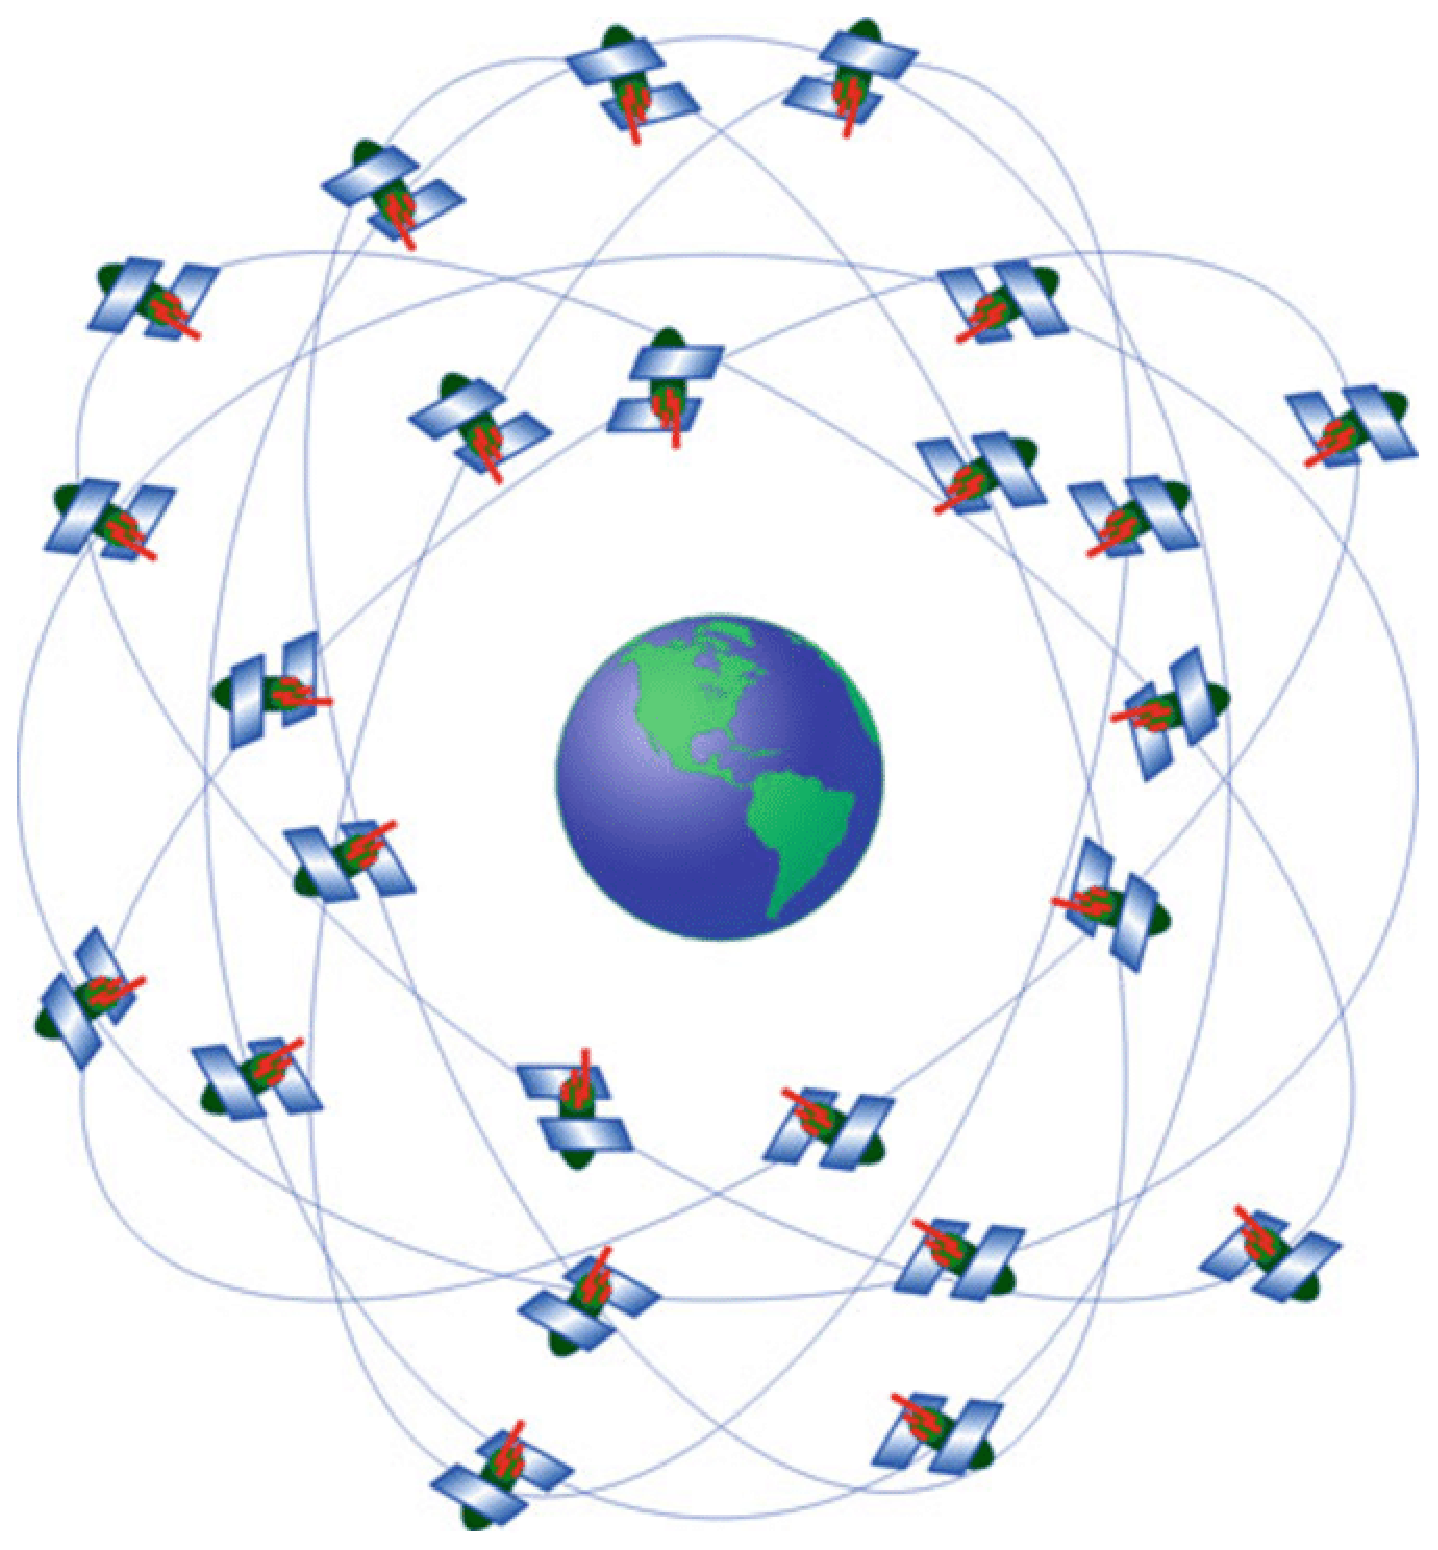
\includegraphics[width=3cm] {fig1-satellites.eps} 
\end{center}
\end{minipage}

\remarque{vert}{E}{Exercice}

\begin{enumerate}


\item Votre récepteur GPS capte la trame suivante : 

\textbf{\$GPGGA,113239.512,4545.47208,N,0449.93164,W,1,8,0.6,3.4,155.3,M,,,*4A"}

\begin{enumerate}

\item Analyser cette trame pour déterminer les paramètres suivants :

\cadrecarre{
\begin{itemize}
\item[$\bullet$] latitude : 
\item[$\bullet$] longitude : 
\item[$\bullet$] latitude : 
\item[$\bullet$] heure d'émission de la trame  : 
\item[$\bullet$] nombre de satellites utilisés  : 
\end{itemize}
}

\end{enumerate}
\item  \begin{enumerate}
\item Ouvrir un navigateur et aller sur \quad  \url{https://www.geoportail.gouv.fr} 
\item Dans le champ de recherche, cliquer sur \textbf{{\LARGE \blue +}} pour accéder à la   recherche avancée.
\item Faire défiler le menu déroulant sur "Coordonnées ".

\item Saisir les coordonnées précédentes afin de découvrir  votre position.
\end{enumerate}
\end{enumerate}
\begin{center}\includegraphics[height=4cm]{fig3_geoportail.eps}\end{center} 
\newpage
{\large \textbf{Partie 2 : Ecriture d'un programme Python }}
\hrulefill


\remarque{orange}{>}{But de cette partie}

Dans cette partie, nous allons coder le travail précédent en Python

\remarque{vert}{?}{Exercice}



\begin{enumerate}
\item Lancer Thonny 
\item Créer un chaine de caractère regroupant la trame reçue par le boitier GPS :
\begin{lstlisting}
trame ="$GPGGA,113239.512,4545.47208,N,0449.93164,W,1,8,0.6,3.4,155.3,M,,,*4A"
\end{lstlisting}
\item Créer une liste en découpant la trame à chaque virgule : 
\begin{lstlisting}
liste = trame.split(',')
\end{lstlisting}
\item Désormais liste[0] contient \textbf{ \$GPGGA}, \quad liste[1] contient  \textbf{113239.512}, \quad liste[2] contient \textbf{4545.47208},  etc.
\begin{enumerate}
\item Saisir la fonction suivante afin de déterminer la latitude d'une liste GPS
\begin{lstlisting}
def latitude(liste):
	valeur = float(liste[2])  		#il s'agit dans l'exemple de 4545.47208
	degre = int(valeur/100)			#chiffres dépassant les centaines  (ici : 45)
	minutes = valeur%100  			#chiffres jusqu'aux centaines (ici : 4545.47208)
	if liste[3]=='N':				#on est au Nord 
	 	return degre + minutes/60    		#la latitude est positive
	else : 
	 	return -degre - minutes/60 			#la latitude est negative
     \end{lstlisting}

\item Exécuter ce programme puis le tester en rajoutant, au choix :
\begin{itemize} 
\item soit dans   le programme, la ligne :
\begin{lstlisting}
print(latitude(liste))
 \end{lstlisting}
 \item soit  dans le Shell, la ligne :
 \begin{lstlisting}
>>> latitude(liste)
 \end{lstlisting}
 \end{itemize}
 
 \item Effectuer le même travail pour la longitude :
 \begin{lstlisting}
def longitude(liste):
	# fonction à compléter

     \end{lstlisting}
\end{enumerate}
\item 
\begin{enumerate}
\item A partir de votre programme, déterminer et afficher les coordonnées GPS relatives à la trame suivante relevée par un boitier GPS :

\textbf{\$GPGGA,071512.34,4851.1791,N,0220.9959,W,1,4,0.6,3.4,62.3,M,,,*0B}
\item Où se situe l'appareil ?

\begin{center}\includegraphics[height=4cm]{fig4_sortie_Thonny_S2.eps}\end{center} 

\end{enumerate}
\end{enumerate}
\end{document}